\section{LTasks}\label{section-ltasks}
To continue the naming scheme of iTasks and mTasks, the proof of concept in this thesis is called LTasks. This section goes into the details of the LTasks library. To prove that the proof of concept is indeed complete for TOP, appendix \ref{appendix} contains some examples in both LTasks and iTasks.

\subsection{Task combinators}
While iTasks provides a lot of combinators, we do not need that for a proof of concept so LTasks includes only the essential combinators and some convenience wrappers around them. Here is the list, along with their operators in LTasks or their equivalent in iTasks:
\begin{itemize}
    \item \lua{constant} (\clean{return} in iTasks)
    \item \lua{step} (\lua{~} in LTasks, \clean{>>*} in iTasks), \lua{stepStable} (\clean{>>-} in iTasks) and \lua{stepButtonStable} (\clean{>>?} in iTasks)
    \item \lua{parallel}, \lua{anyTask}, \lua{parallelAnd} (\lua{&} in LTasks, \clean{-&&-} in iTasks), \lua{parallelOr} (\lua{|} in LTasks, \clean{-||-} in iTasks), \lua{parallelLeft} (\clean{-||} in iTasks) and \lua{parallelRight} (\clean{||-} in iTasks)
    \item \lua{transform} and \lua{transformValue} (\clean{@} in iTasks)
\end{itemize}

These are the most important functions for building a TOP system, as we defined in section \ref{section-top-lua}.

\subsubsection{Step}
\dots

\subsubsection{Parallel}
\dots

\subsubsection{Custom operators}
In Clean it is common to define lots of operators. For example, there are eight different operators for variations of the step combinator. Lua does allow for changing the behaviour of the standard operators, but only up to a point. For example, the result of the comparison operators like \lua{<} is always converted to a boolean \cite{luareferencemanual}. Perhaps the most notable library that uses operators with custom behaviour is LPeg\footnote{\url{http://www.inf.puc-rio.br/~roberto/lpeg/}}. It is not so common to redefine the behaviour of the operators in Lua, so LTasks only uses three operators: \lua{~}, \lua{&} and \lua{|}. Originally the operator for \lua{step} was \lua{..}, which more resembles its original meaning (concatenation, putting strings after each other). It was changed because its right-associativity does not play well with chaining multiple operators.

\subsection{Type matching}
Instead of implementing a type matching algorithm defined in section \ref{section-combinators-type-matching}, we just used the Typed\footref{footnote-typed} library to compare types, which is very strict in what it matches. There is a Lua library for matching data structures called Tamale\footnote{\url{https://luarocks.org/modules/luarocks/tamale}}, however it is not made for matching types so it is also strict in what it matches. Therefore we do not use Tamale. \dots

\subsection{Editors}
\dots

\subsection{User Interface with LTUI}
For simplicity with working with LTUI, I decided to only ever have one UI element of a type at once. Instead of creating a new element every time, the old one is re-used, displayed, and hidden when no longer needed. These re-used elements are defined and created once in \lua{ltuiApp.lua}.
The module \lua{ltuiElements.lua} provides functions that use these reusable elements and set the contents like the task name or the current value.
\lua{ltuiEditor.lua} is the module that then converts these editors into tasks so they can be used with TOP. This module provides the same functions with the same parameters as \lua{terminalEditor.lua}, which provides editors that use standard I/O as a command-line interface instead of a textual UI.

\begin{figure}
    \centering
    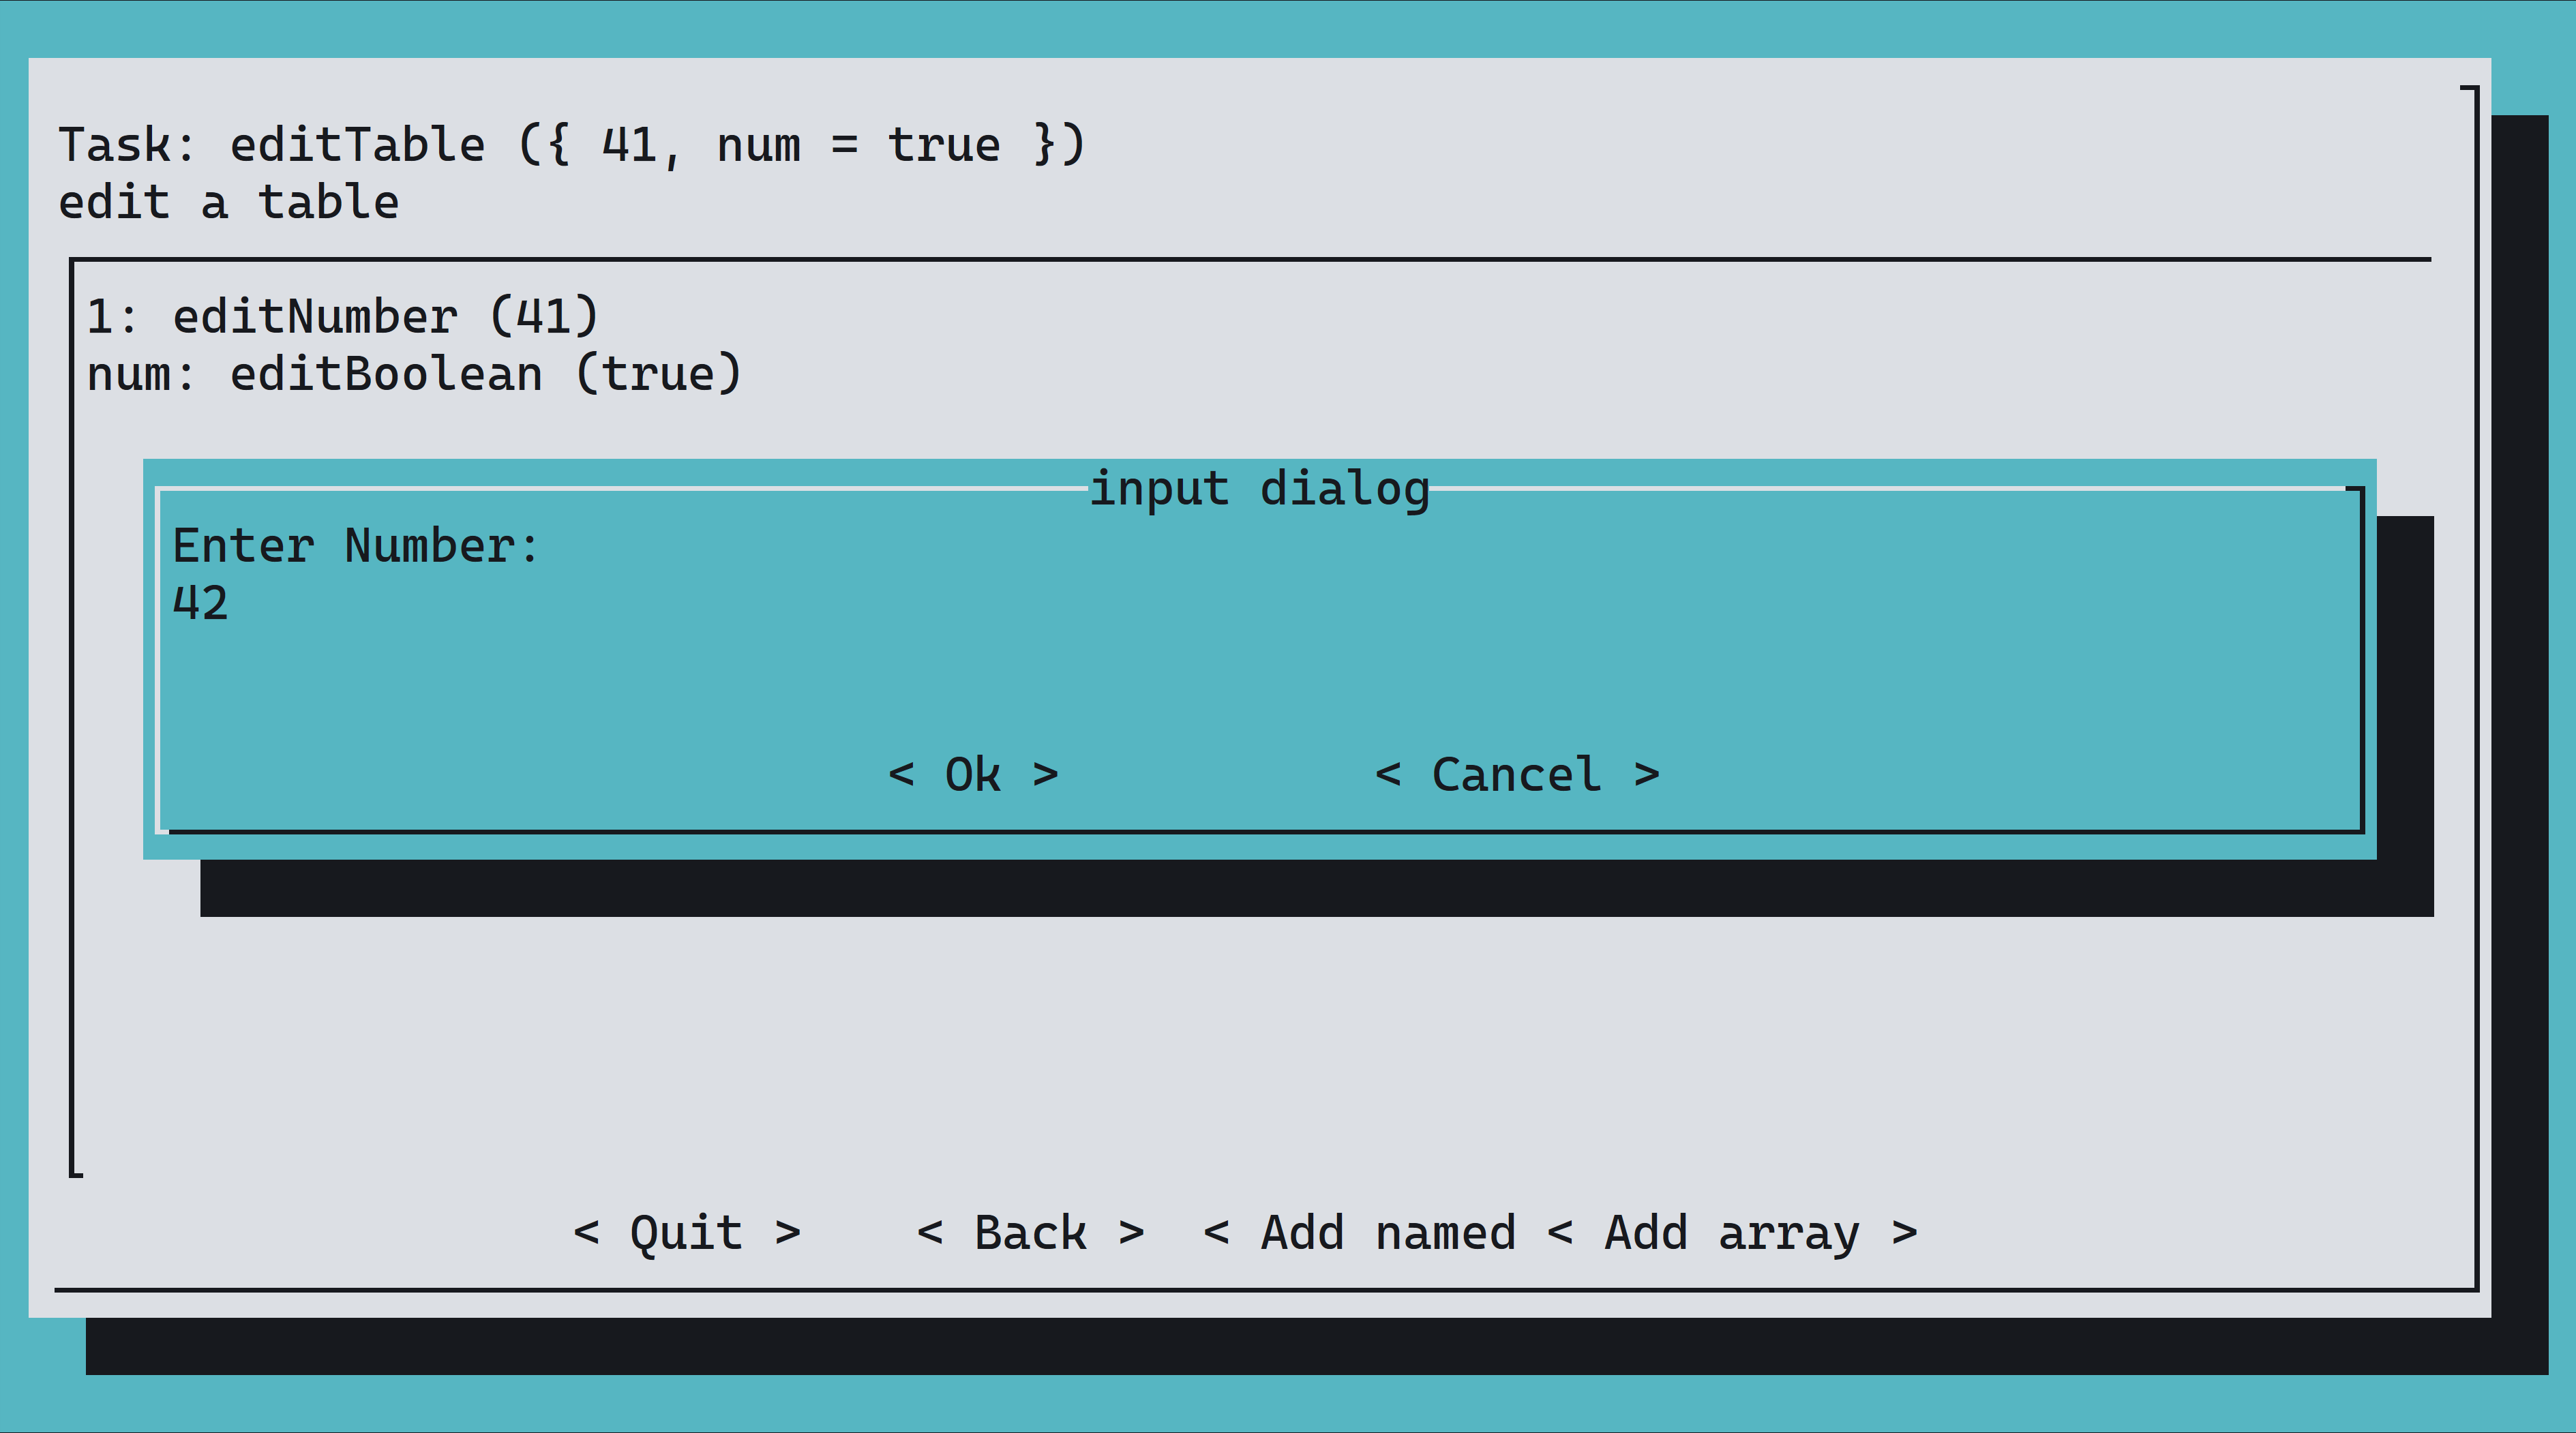
\includegraphics[width=\textwidth]{img/screenshot-ltui.png}
    \caption{The textual UI showing a table editor in the background with a number input dialog in the foreground.}
    \label{fig:ltask_ui}
\end{figure}
